\documentclass{beamer}

%\author[D. Abercrombie]{
\author[Workflow Team]{
  \underline{Daniel Abercrombie}, \emph{MIT} \\
  Allison Reinsvold Hall, \emph{Notre Dame} \\
  Paola Katherine Rozo Bernal, \emph{CERN} \\
  Jean-Roch Vlimant, \emph{CalTech}
}

\title{\bf \sffamily Machine Learning for Workflow Handling}
\date{July 5, 2017}

\usecolortheme{dove}

\usepackage[absolute,overlay]{textpos}
\usefonttheme{serif}
\usepackage{appendixnumberbeamer}
\usepackage{hyperref}
\usepackage[english]{babel}
\usepackage{amsmath}
\setbeamerfont{frametitle}{size=\Large,series=\bf\sffamily}
\setbeamertemplate{frametitle}[default][center]

\setbeamertemplate{navigation symbols}{}
\usepackage{color}
\setbeamertemplate{footline}[text line]{\parbox{1.083\linewidth}{\footnotesize \hfill \insertshortauthor \hfill \insertpagenumber /\inserttotalframenumber}}
\setbeamertemplate{headline}[text line]{\parbox{1.083\linewidth}{\footnotesize \hspace{-0.083\linewidth} \textcolor{blue}{\sffamily \insertsection \hfill \insertsubsection}}}

\IfFileExists{/Users/dabercro/GradSchool/Presentations/MIT-logo.pdf}
             {\logo{\includegraphics[height=0.5cm]{/Users/dabercro/GradSchool/Presentations/MIT-logo.pdf}}}
             {\logo{\includegraphics[height=0.5cm]{/home/dabercro/MIT-logo.pdf}}}

\usepackage{changepage}

\newcommand{\beginbackup}{
  \newcounter{framenumbervorappendix}
  \setcounter{framenumbervorappendix}{\value{framenumber}}
}
\newcommand{\backupend}{
  \addtocounter{framenumbervorappendix}{-\value{framenumber}}
  \addtocounter{framenumber}{\value{framenumbervorappendix}}
}

\graphicspath{{figs/}}

\begin{document}

\begin{frame}[nonumbering]
  \titlepage
\end{frame}

\begin{frame}
  \frametitle{Introduction}

  \begin{itemize}
  \item During central production of datasets,
    we sometimes get errors such as
    missing files or high memory usage.
  \item An operator must look at the error codes and decide what action to take on the workflow.
  \item Some errors are easy to understand, and there are automated responses.
  \item An algorithm that encompassed all possible patterns that we can anticipate
    would be difficult or impossible to maintain.
  \item Machine learning is a natural solution.
  \end{itemize}

\end{frame}

\begin{frame}
  \frametitle{Defining a Model}

  \begin{itemize}
  \item For each workflow,
    we know the number of times each possible error code is thrown at each site.
  \item This leads to a simple matrix of number of error codes times the number of sites,
    with each element being the number of matching errors.
  \item Another feature considered is the site status at the time of the error
    (enabled, disabled, or in drain).
  \item We just split these into ``good'' and ``bad'' site status,
    so there is a factor of two more features.
  \end{itemize}

\end{frame}

\begin{frame}
  \frametitle{Example of Features}

  The color of each site corresponds to its status. \\
  \vspace{-6pt}
  {\tiny(White sites are not tracked by dashboard being used, so they're counted as ``good.'')}
  \vspace{6pt}

  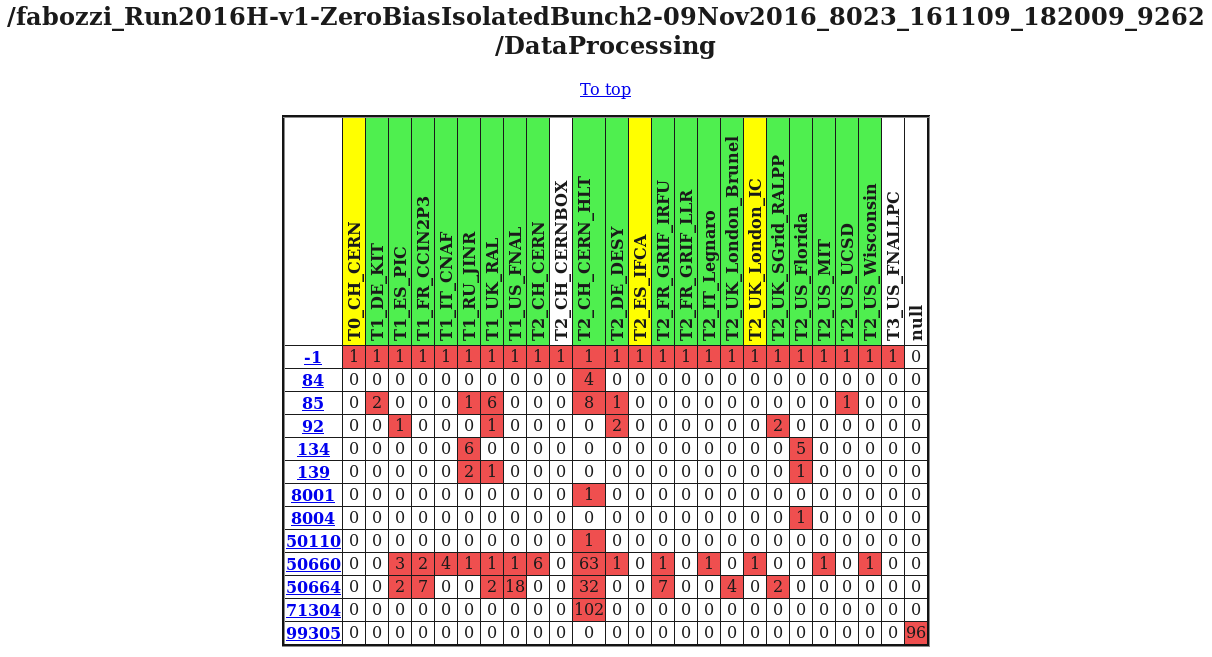
\includegraphics[width=\linewidth]{original.png}

  Note the largest 4 error codes: 71304, 50660, and 50664 at T2\_CH\_CERN\_HLT and 99305.
  We will come back to those.

\end{frame}

\begin{frame}
  \frametitle{Unsupervised Learning Before the Operator}

  \begin{itemize}
  \item First way we help the operator is to group similar error-type workflows together.
  \item Multiple workflows can then be acted on at the same time.
  \item To make the cluster characteristics stable,
    we include workflow error patterns and site statuses stored over the past few months.
  \item We are using K-Means clustering.
    (\url{http://scikit-learn.org/stable/modules/clustering.html#k-means})
  \end{itemize}

\end{frame}

\begin{frame}
  \frametitle{Quick Definition of K-Means Clustering}

  \begin{itemize}
  \item Each point is inside the cluster corresponding to the nearest centroid.
  \item The centroid location is placed where the variance
    (the sum of the squared distances from the centroid)
    of the entire cluster is minimized.
  \end{itemize}

  \begin{center}
    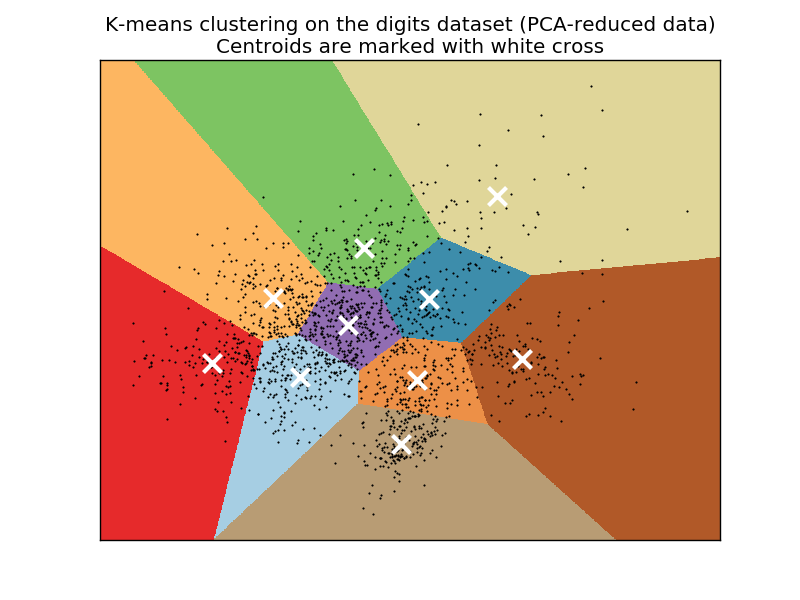
\includegraphics[width=0.6\linewidth]{kmeans.png} \\
    \vspace{-6pt}
    \textcolor{blue}{Image taken from scikit-learn.org.}
  \end{center}
\end{frame}

\begin{frame}
  \frametitle{Vector Compression}

  \begin{itemize}
  \item Instead of errors times sites, we are using errors plus sites number of features.
  \item This helps group together similar errors,
    even if spread across sites.
  \item Because of potential large geometric distances due to large number of errors,
    we also compress error and site phase space.
  \end{itemize}

  \begin{gather}
  \text{distance from origin} = \frac{d}{\sqrt{2}} +
      2 w \left(\frac{|\vec{v}|}{|\vec{v}| + m} - 0.5\right)
  \end{gather}

  \hspace{0.2\linewidth}
  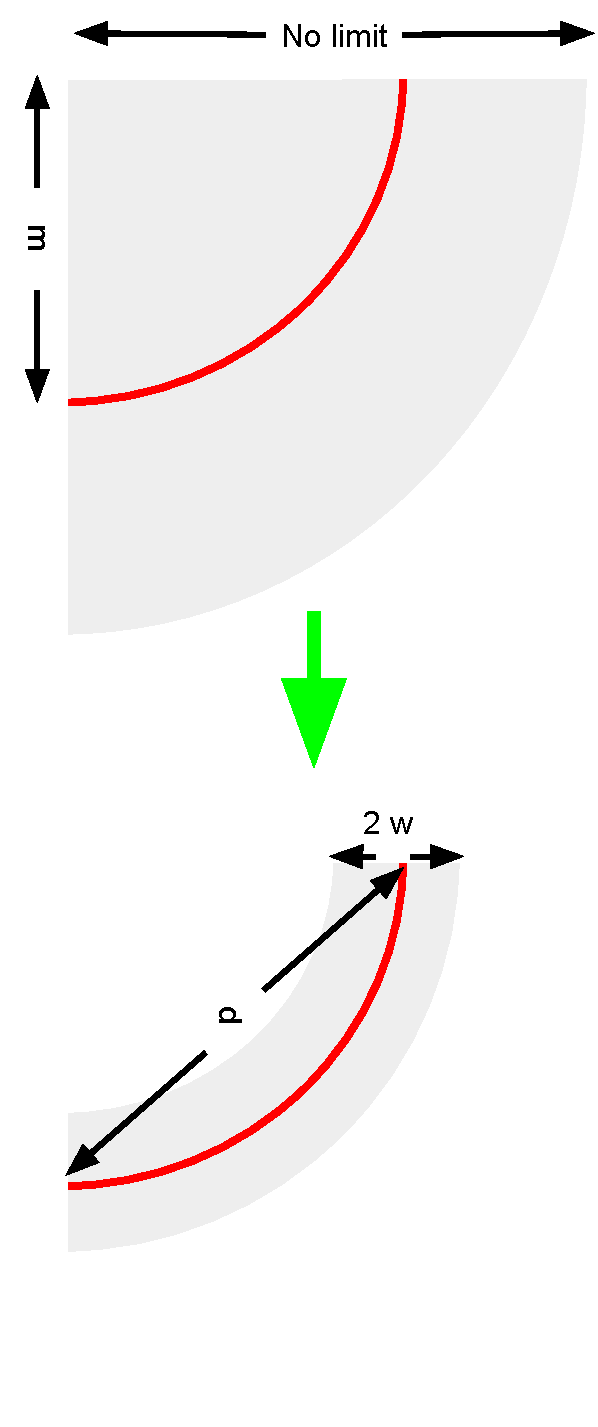
\includegraphics[height=0.6\linewidth, angle=90]{compress.pdf}

\end{frame}

\begin{frame}
  \frametitle{An Obviously Similar Workflow}

  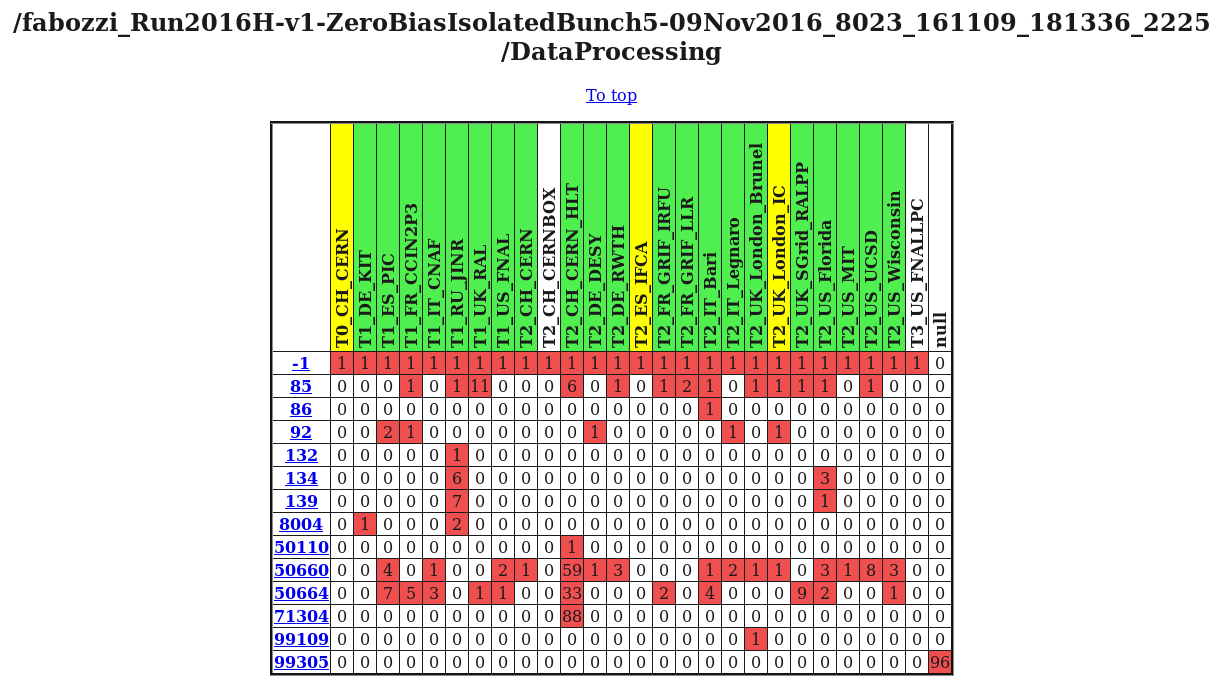
\includegraphics[width=\linewidth]{similar.png}

  \begin{itemize}
  \item This workflow has the same four top error codes as before:
    71304, 50660, and 50664 at T2\_CH\_CERN\_HLT and 99305.
  \item From the task name itself, we can also see that the workflows are similar.
  \end{itemize}

\end{frame}

\begin{frame}
  \frametitle{A Less Obvious Similar Workflow}

  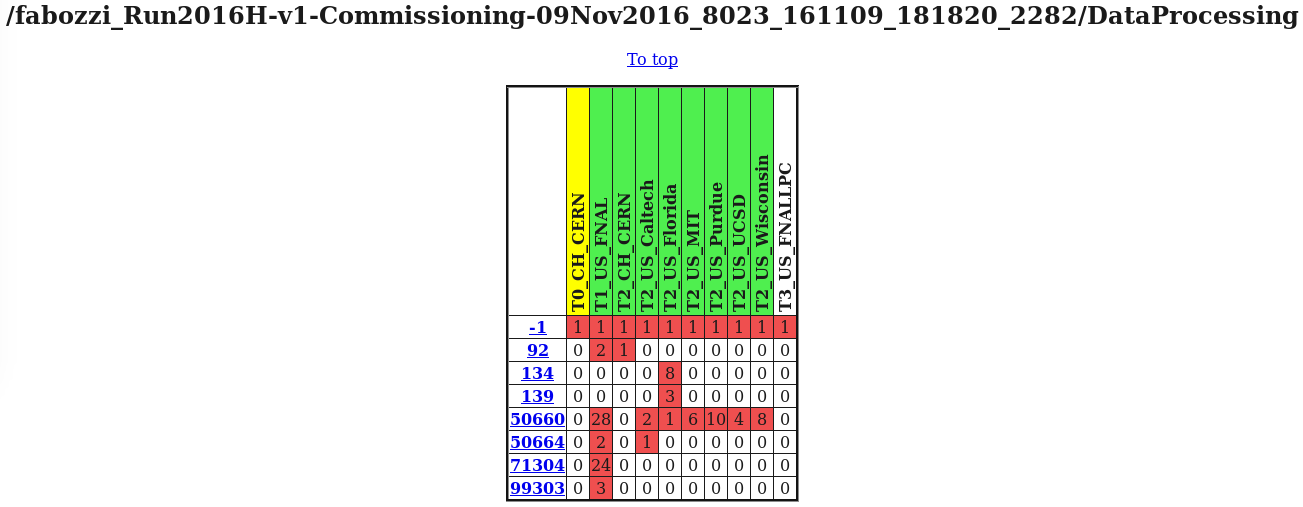
\includegraphics[width=\linewidth]{fnal_same_err.png}

  \begin{itemize}
  \item This workflow might not look the exact same at a first glance,
    but the 71304 and 50660 errors at a different site are likely from similar causes.
  \item Our algorithm clusters this with the previously shown workflows
    for the operator to review simultaneously.
  \end{itemize}

\end{frame}

\begin{frame}
  \frametitle{Operator View}

  \begin{itemize}
  \item A prototype here shows errors codes for each workflow.
  \item Each color of the pie chart is a different site.
  \item The size of the pie charts corresponds to the number of errors.
  \end{itemize}

  \hspace{0.25\linewidth}
  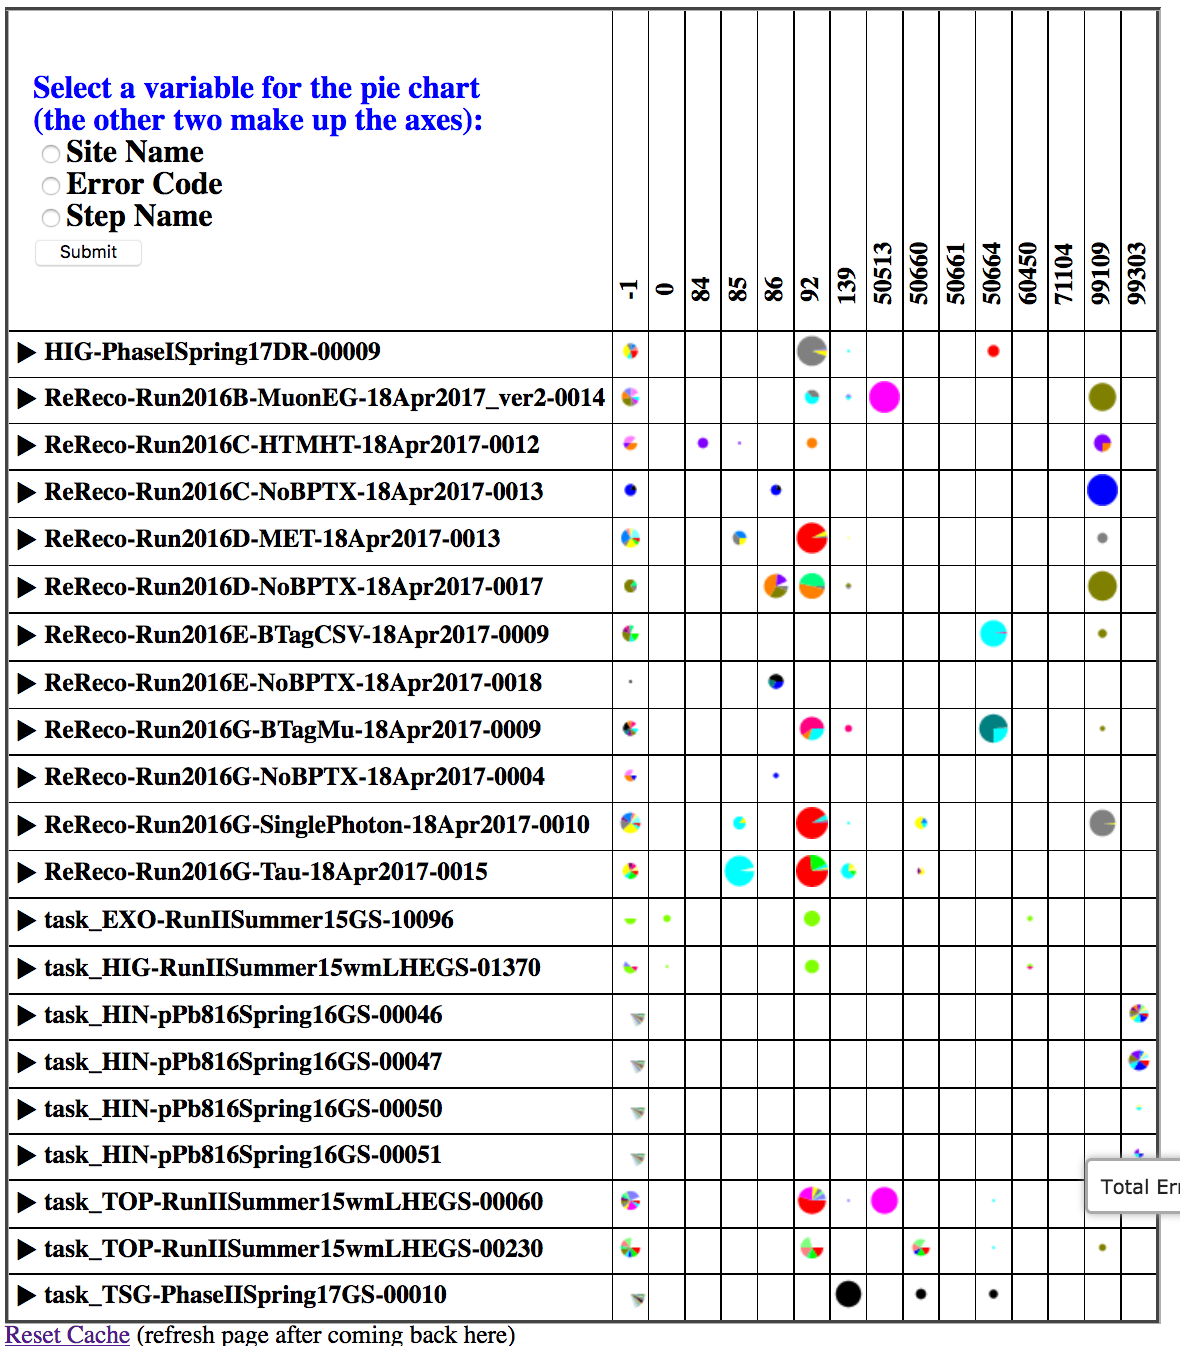
\includegraphics[width=0.5\linewidth]{Global.png}

\end{frame}

\begin{frame}
  \frametitle{Interlude}

  Short version: \\
  We are pulling in information from Request Manager (workflow parameters)
  and WMStats servers (errors thrown) to inform the operator who has to make a decision.

  \vspace{12pt}

  All of this information can be used for training, but
  for now, we are using WMStats errors exclusively for this purpose.

\end{frame}

\begin{frame}
  \frametitle{Gathering Operator Actions}

  \begin{itemize}
  \item We are trying to limit and enumerate possible operator actions.
  \item Turn command line script into series of options.
  \item Example actions would be to kill and clone jobs,
    or to recover partially complete jobs (ACDC).
  \item Farther parameters to train on are: \\
    job splitting, enabling XRootD,  and requested memory
  \end{itemize}
\end{frame}

\begin{frame}
  \frametitle{Gathering Operator Actions}

  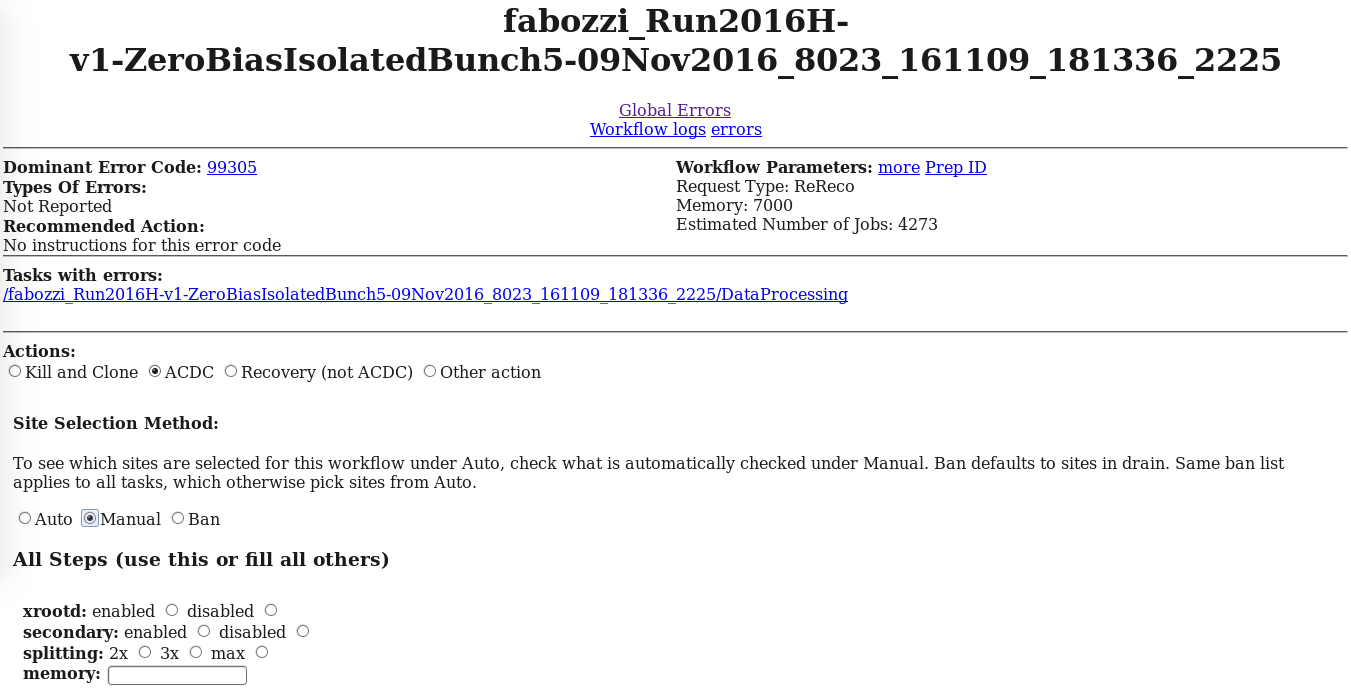
\includegraphics[width=\linewidth]{decision.png}

\end{frame}

\begin{frame}
  \frametitle{First Passes with Actions}

  \begin{itemize}
  \item Very much in progress as we collect operator actions.
  \item Using full feature vectors without compression, we dump into a neural net.
  \item Number of features is \# Error codes $\times$ \# Sites $\times 2 \approx 10000$.
  \item Parameters for classifier are just the defaults from
    \texttt{sklearn.neural\_network.MLPClassifier}: \\
    \url{http://scikit-learn.org/stable/modules/neural_networks_supervised.html#classification}
  \end{itemize}

  In the following example, we use the 10000 features to decide between 2 classes.

\end{frame}

\begin{frame}
  \frametitle{First Passes with Actions}
  \begin{itemize}
  \item Predicting action (ACDC vs. clone) is 97\% (109/112) for training sample
    and 82\% (84/102) for test sample.
  \item Below is a plot of the first two principle components.
  \item PCA does not seem to cause much separation on its own.
  \end{itemize}

  \begin{columns}
    \begin{column}{0.5\linewidth}
      \centering
      \textcolor{blue}{First two Principle Components} \\
      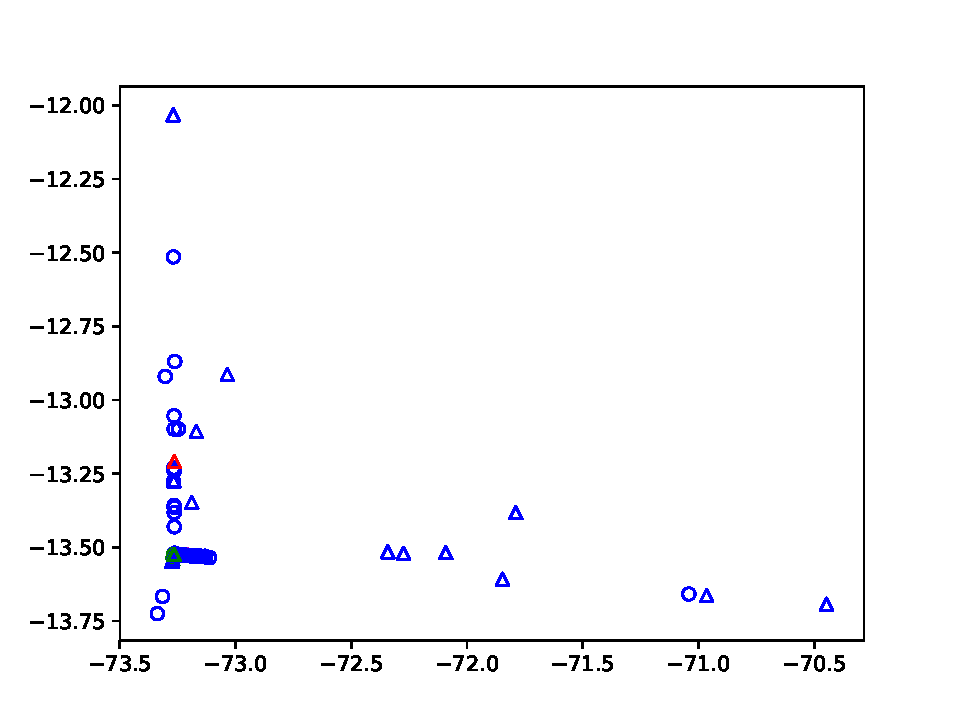
\includegraphics[width=\linewidth]{full.pdf}
    \end{column}
    \begin{column}{0.5\linewidth}
      \centering
      \textcolor{blue}{Zoomed a bit} \\
      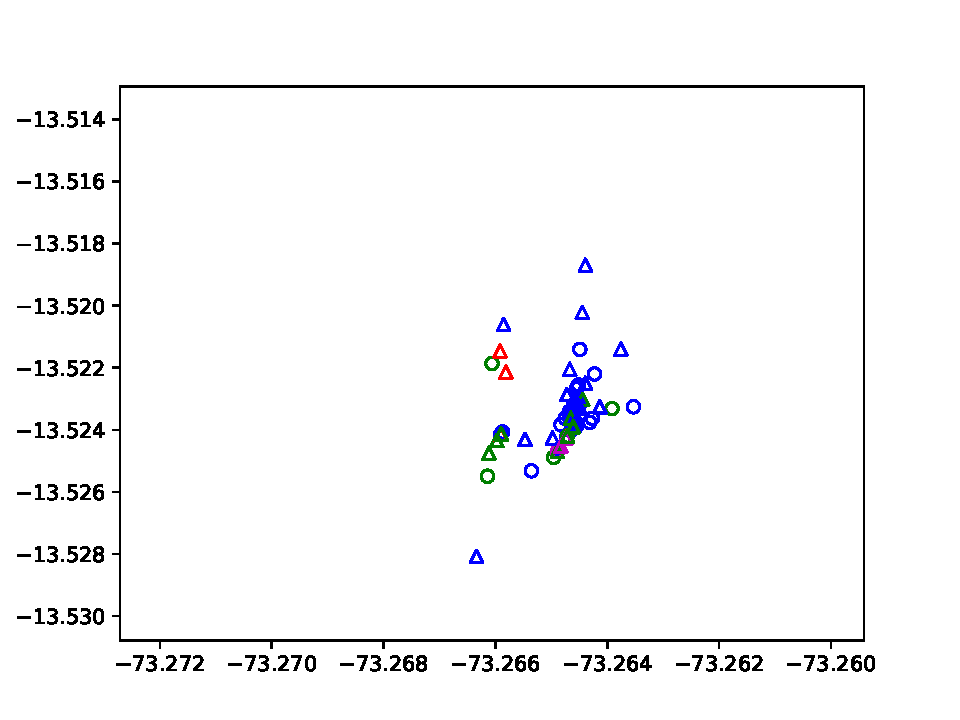
\includegraphics[width=\linewidth]{zoomed.pdf}
      \end{column}
  \end{columns}

  {\small
  \begin{itemize}
  \item Circles are training data, triangles are test data
  \item \textcolor{blue}{Blue} correctly identified recovery, \textcolor{green}{green} is clone
  \item \textcolor{magenta}{Magenta} recovery not identifed, and \textcolor{red}{red} is clone
  \end{itemize}
  }

\end{frame}

\begin{frame}
  \frametitle{Conclusions}

  \begin{itemize}
  \item Prototype of interface for operator was built with discrete options
  \item Capable of clustering workflows with similar errors
  \item We are recording the actions taken in a manner that can be trained
  \item \textcolor{red}{[Work in progress]:}
    We have started experimenting with predicting actions
  \end{itemize}
\end{frame}

%\beginbackup
%
%\begin{frame}
%  \frametitle{Backup Slides}
%\end{frame}
%
%\backupend

\end{document}

